\section{程序的机器级表示}

\subsection{汇编代码基础}
\subsubsection{寄存器}
\begin{table}[H]
    \centering
    \begin{tabular}{|c|c|c|c|c|}
        \hline
        \multicolumn{4}{|c|}{\textbf{寄存器}} & \multirow{2}{*}{\textbf{备注}}                                                \\
        \cline{1-4}
        64位                                & 32位                          & 16位    & 8位     &                            \\
        \hline
        \%rax                              & \%eax                        & \%ax   & \%al   & 函数返回值(accumulator)         \\
        \hline
        \%rbx                              & \%ebx                        & \%bx   & \%bl   & 基址寄存器(base)                \\
        \hline
        \%rcx                              & \%ecx                        & \%cx   & \%cl   & 计数器(counter)               \\
        \hline
        \%rdx                              & \%edx                        & \%dx   & \%dl   & 数据寄存器(data)                \\
        \hline
        \%rsi                              & \%esi                        & \%si   & \%sil  & 源变址寄存器(source index)       \\
        \hline
        \%rdi                              & \%edi                        & \%di   & \%dil  & 目的变址寄存器(destination index) \\
        \hline
        \%rsp                              & \%esp                        & \%sp   & \%spl  & 堆栈指针寄存器(stack pointer)     \\
        \hline
        \%rbp                              & \%ebp                        & \%bp   & \%bpl  & 基址指针寄存器(base pointer)      \\
        \hline
        \%r8                               & \%r8d                        & \%r8w  & \%r8b  & /                          \\
        \hline
        \%r9                               & \%r9d                        & \%r9w  & \%r9b  & /                          \\
        \hline
        \%r10                              & \%r10d                       & \%r10w & \%r10b & /                          \\
        \hline
        \%r11                              & \%r11d                       & \%r11w & \%r11b & /                          \\
        \hline
        \%r12                              & \%r12d                       & \%r12w & \%r12b & /                          \\
        \hline
        \%r13                              & \%r13d                       & \%r13w & \%r13b & /                          \\
        \hline
        \%r14                              & \%r14d                       & \%r14w & \%r14b & /                          \\
        \hline
        \%r15                              & \%r15d                       & \%r15w & \%r15b & /                          \\
        \hline
    \end{tabular}
\end{table}

当指令以寄存器作为目标时,生成小于 8 字节结果时,寄存器有两条规则:
\begin{itemize}
    \item 生成 1 字节和 2 字节数字的指令会保持剩下的字节不变。
    \item 生成 4 字节数字的指令会把高位 4 个字节置为 0 。
\end{itemize}
\subsubsection{操作数}
\begin{table}[H]
    \centering
    \begin{tabular}{|c|c|c|}
        \hline
        \textbf{操作数类型} & \textbf{格式}      & \textbf{数值}                        \\
        \hline
        寄存器            & $r_a$            & $R[r_a]$                           \\
        \hline
        立即数            & $\$Imm$          & $Imm$                              \\
            \hline
        存储器            & $Imm(r_b,r_i,s)$ & $M[Imm + R[r_b] + R[r_i] \cdot s]$ \\
        \hline
    \end{tabular}
\end{table}

注意:
\begin{itemize}
    \item 比例因子$s$必须是1、2、4或者8。
    \item 基址和变址寄存器都必须是64位寄存器。
\end{itemize}

\subsubsection{基础指令}
\paragraph{数据传送指令}
\begin{table}[H]
    \centering
    \begin{tabular}{|c c|c|c|}
        \hline
        \multicolumn{2}{|c|}{\textbf{指令}} & \textbf{效果} & \textbf{描述}                                       \\
        \hline
        MOV                               & S, D        & $D \leftarrow S$               & 传送               \\
        \hline
        moveb                             &             &                                & 传送字节             \\
        movew                             &             &                                & 传送字              \\
        movel                             &             &                                & 传送双字             \\
        moveq                             &             &                                & 传送四字             \\
        moveabsq                          & I, R        & $R \leftarrow I$               & 传送绝对四字           \\
        \hline
        MOVZ                              & S, R        & R $\leftarrow$ 零扩展(S)          & 以零扩展进行传送         \\
        \hline
        movezbw                           &             &                                & 将做了零扩展的字节传送到字    \\
        movezbl                           &             &                                & 将做了零扩展的字节传送到双字   \\
        movezwl                           &             &                                & 将做了零扩展的字传送到双字    \\
        movezbq                           &             &                                & 将做了零扩展的字节传送到四字   \\
        movezwq                           &             &                                & 将做了零扩展的字传送到四字    \\
        \hline
        MOVS                              & S, R        & R $\leftarrow$ 符号扩展(S)         & 以符号扩展进行传送        \\
        \hline
        movesbw                           &             &                                & 将做了符号扩展的字节传送到字   \\
        movesbl                           &             &                                & 将做了符号扩展的字节传送到双字  \\
        moveswl                           &             &                                & 将做了符号扩展的字传送到双字   \\
        movesbq                           &             &                                & 将做了符号扩展的字节传送到四字  \\
        moveswq                           &             &                                & 将做了符号扩展的字传送到四字   \\
        moveslq                           &             &                                & 将做了符号扩展的双字传送到四字  \\
        cltq                              &             & \%rax $\leftarrow$ 符号扩展(\%eax) & 把\%eax符号扩展到\%rax \\
        \hline
    \end{tabular}
\end{table}

注意:
\begin{itemize}
    \item movl指令以寄存器作为目的时,它会把该寄存器的高位4字节设置为0。
    \item 常规的movq指令只能以表示为32位补码数字的立即数作为源操作数,然后把这个值符号扩展得到64位的值,放到目的位置。
    \item movabsq指令能够以任意64位立即数值作为源操作数,并且只能以寄存器作为目的。
\end{itemize}
\paragraph{压栈弹栈指令}
\begin{table}[H]
    \centering
    \begin{tabular}{|c c|c|c|}
        \hline
        \multicolumn{2}{|c|}{\textbf{指令}} & \textbf{效果}        & \textbf{描述}                                                \\
        \hline
        \multirow{2}{*}{pushq}            & \multirow{2}{*}{S} & $R[\%rsp] \leftarrow R[\%rsp]-8$ & \multirow{2}{*}{将四字压入栈} \\
                                          &                    & $M[R[\%rsp]] \leftarrow S$       &                         \\
        \hline
        \multirow{2}{*}{popq}             & \multirow{2}{*}{D} & $D \leftarrow M[R[\%rsp]]$       & \multirow{2}{*}{将四字弹出栈} \\
                                          &                    & $R[\%rsp] \leftarrow R[\%rsp]+8$ &                         \\
        \hline
    \end{tabular}
\end{table}

\paragraph{算术运算指令}
\begin{table}[H]
    \centering
    \begin{tabular}{|c c|c|c|}
        \hline
        \multicolumn{2}{|c|}{\textbf{指令}} & \textbf{效果}        & \textbf{描述}                                                           \\
        \hline
        leaq                              & S, D               & $D \leftarrow \&S$                           & 加载有效地址                 \\
        \hline
        inc                               & D                  & $D \leftarrow D + 1$                         & 加1                     \\
        dec                               & D                  & $D \leftarrow D - 1$                         & 减1                     \\
        neg                               & D                  & $D \leftarrow -D$                            & 取负                     \\
        not                               & D                  & $D \leftarrow \sim D$                        & 取补                     \\
        \hline
        add                               & S, D               & $D \leftarrow D + S$                         & 加                      \\
        sub                               & S, D               & $D \leftarrow D - S$                         & 减                      \\
        imul                              & S, D               & $D \leftarrow D * S$                         & 乘                      \\
        xor                               & S, D               & $D \leftarrow D \oplus S$                    & 异或                     \\
        and                               & S, D               & $D \leftarrow D \,\&\, S$                    & 与                      \\
        or                                & S, D               & $D \leftarrow D \,\,|\,\, S$                 & 或                      \\
        \hline
        sal                               & k, D               & $D \leftarrow D << k$                        & 左移                     \\
        shl                               & k, D               & $D \leftarrow D << k$                        & 左移                     \\
        sar                               & k, D               & $D \leftarrow D >>_A k$                      & 算术右移                   \\
        shr                               & k, D               & $D \leftarrow D >>_L k$                      & 逻辑右移                   \\
        \hline
        imulq                             & S                  & $R[\%rdx]:R[\%rax] \leftarrow S * R[\%rax]$  & 有符号全乘法                 \\
        mulq                              & S                  & $R[\%rdx]:R[\%rax] \leftarrow S * R[\%rax]$  & 无符号全乘法                 \\
        \hline
        cqto                              &                    & $R[\%rdx:\%rax] \leftarrow$ 符号扩展$(R[\%rax])$ & 转换为八字                  \\
        \hline
        \multirow{2}{*}{idivq}            & \multirow{2}{*}{S} & $R[\%rdx] \leftarrow R[\%rdx:\%rax] \mod S$  & \multirow{2}{*}{有符号除法} \\
                                          &                    & $R[\%rax] \leftarrow R[\%rdx:\%rax] \div S$  &                        \\
        \hline
        \multirow{2}{*}{divq}             & \multirow{2}{*}{S} & $R[\%rdx] \leftarrow R[\%rdx:\%rax] \mod S$  & \multirow{2}{*}{无符号除法} \\
                                          &                    & $R[\%rax] \leftarrow R[\%rdx:\%rax] \div S$  &                        \\
        \hline
    \end{tabular}
\end{table}

注意:
\begin{itemize}
    \item 移位指令只有一个操作数D时,代表将D的值左移或右移1位。
    \item 位移指令的移位量只能存放在单字节寄存器\%cl中,或者作为立即数给出。
\end{itemize}

\subsection{控制}
\subsubsection{条件码}
\paragraph{条件码定义}
\begin{table}[H]
    \centering
    \begin{tabular}{|c|c|c|}
        \hline
        \textbf{标志} & \textbf{描述}   & \textbf{含义}   \\
        \hline
        ZF          & Zero Flag     & 结果为0时置1,否则为0  \\
        \hline
        SF          & Sign Flag     & 结果为负时置1,否则为0  \\
        \hline
        OF          & Overflow Flag & 有符号溢出时置1,否则为0 \\
        \hline
        CF          & Carry Flag    & 无符号溢出时置1,否则为0 \\
        \hline
    \end{tabular}
\end{table}

注意:
\begin{itemize}
    \item leaq指令不改变任何条件码,因为它是用来进行地址计算的。
    \item 对于XOR,进位标志和溢出标志会设置成0。
    \item 对于移位操作,进位标志将设置为最后一个被移出的位,而溢出标志设置为0。
    \item INC和DEC指令会设置溢出和零标志,但是不会改变进位标志。
\end{itemize}
\paragraph{条件码访问}
\begin{table}[H]
    \centering
    \begin{tabular}{|c c|c|c|}
        \hline
        \multicolumn{2}{|c|}{\textbf{指令}} & \textbf{效果}  & \textbf{描述}                                             \\
        \hline
        CMP                               & $S_1$, $S_2$ & $S_2-S_1$                                     & 比较      \\
        \hline
        TEST                              & $S_1$, $S_2$ & $S_1 \& S_2$                                  & 测试      \\
        \hline
        SET                               & D            &                                               & 设置单字节   \\
        \hline
        sete/setz                         & D            & $D \leftarrow ZF$                             & 相等/零    \\
        setne/setnz                       & D            & $D \leftarrow \sim ZF$                        & 不等/非零   \\
        \hline
        sets                              & D            & $D \leftarrow SF$                             & 负数      \\
        setns                             & D            & $D \leftarrow D \sim SF$                      & 非负数     \\
        \hline
        setg/setnle                       & D            & $D \leftarrow \sim (SF \oplus OF) \& \sim ZF$ & 有符号大于   \\
        setge/setnl                       & D            & $D \leftarrow \sim (SF \oplus OF)$            & 有符号大于等于 \\
        setl/setnge                       & D            & $D \leftarrow SF \oplus OF$                   & 有符号小于   \\
        setle/setng                       & D            & $D \leftarrow (SF \oplus OF) | ZF$            & 有符号小于等于 \\
        \hline
        seta/setnbe                       & D            & $D \leftarrow \sim CF \& \sim ZF$             & 无符号大于   \\
        setae/setnb                       & D            & $D \leftarrow \sim CF$                        & 无符号大于等于 \\
        setb/setnae                       & D            & $D \leftarrow CF$                             & 无符号小于   \\
        setbe/setna                       & D            & $D \leftarrow CF | ZF$                        & 无符号小于等于 \\
        \hline
    \end{tabular}
\end{table}

\subsubsection{跳转指令}
\begin{table}[H]
    \centering
    \begin{tabular}{|c c|c|c|}
        \hline
        \multicolumn{2}{|c|}{\textbf{指令}} & \textbf{跳转条件} & \textbf{描述}                                \\
        \hline
        jmp                               & Label         & 1                                & 直接跳转    \\
        jmp                               & *Operand      & 1                                & 间接跳转    \\
        \hline
        je/jz                             & Label         & $ZF$                             & 相等/零    \\
        jne/jnz                           & Label         & $\sim ZF$                        & 不等/非零   \\
        \hline
        js                                & Label         & $SF$                             & 负数      \\
        jns                               & Label         & $\sim SF$                        & 非负数     \\
        \hline
        jg/jnle                           & Label         & $\sim (SF \oplus OF) \& \sim ZF$ & 有符号大于   \\
        jge/jnl                           & Label         & $\sim (SF \oplus OF)$            & 有符号大于等于 \\
        jl/jnge                           & Label         & $SF \oplus OF$                   & 有符号小于   \\
        jle/jng                           & Label         & $(SF \oplus OF) | ZF$            & 有符号小于等于 \\
        \hline
        ja/jnbe                           & Label         & $\sim CF \& \sim ZF$             & 无符号大于   \\
        jae/jnb                           & Label         & $\sim CF$                        & 无符号大于等于 \\
        jb/jnae                           & Label         & $CF$                             & 无符号小于   \\
        jbe/jna                           & Label         & $CF | ZF$                        & 无符号小于等于 \\
        \hline
    \end{tabular}
\end{table}

\subsubsection{条件分支}
\paragraph{条件控制}
\begin{lstlisting}[style=CStyle]
t = ...;  // test-expr
if (!t)
    goto false;
...  // then-statement
goto done;
false:
    ...  // else-statement
done:
    ...
\end{lstlisting}
\paragraph{条件传送}
\begin{lstlisting}[style=CStyle]
/* result = test-expr ? then-expr : else-expr; */
t = ...;  // test-expr
result = ...;  // then-expr
eval = ...;  // else-expr
if (!t) result = eval;
\end{lstlisting}

注意,无论测试结果如何,then-expr 和 else-expr 都会被求值。如果这两个表达式中的任意一个可能产生错误条件或者副作用,就会导致非法的行为。

\begin{table}[H]
    \centering
    \begin{tabular}{|c c|c|c|}
        \hline
        \multicolumn{2}{|c|}{\textbf{指令}} & \textbf{传送条件} & \textbf{描述}                                \\
        \hline
        cmove/cmovz                       & S, R          & $ZF$                             & 相等/零    \\
        cmovne/cmovnz                     & S, R          & $\sim ZF$                        & 不等/非零   \\
        \hline
        cmovs                             & S, R          & $SF$                             & 负数      \\
        cmovns                            & S, R          & $\sim SF$                        & 非负数     \\
        \hline
        cmovg/cmovnle                     & S, R          & $\sim (SF \oplus OF) \& \sim ZF$ & 有符号大于   \\
        cmovge/cmovnl                     & S, R          & $\sim (SF \oplus OF)$            & 有符号大于等于 \\
        cmovl/cmovnge                     & S, R          & $SF \oplus OF$                   & 有符号小于   \\
        cmovle/cmovng                     & S, R          & $(SF \oplus OF) | ZF$            & 有符号小于等于 \\
        \hline
        cmova/cmovnbe                     & S, R          & $\sim CF \& \sim ZF$             & 无符号大于   \\
        cmovae/cmovnb                     & S, R          & $\sim CF$                        & 无符号大于等于 \\
        cmovb/cmovnae                     & S, R          & $CF$                             & 无符号小于   \\
        cmovbe/cmovna                     & S, R          & $CF | ZF$                        & 无符号小于等于 \\
        \hline
    \end{tabular}
\end{table}

源和目的的值可以是 16 位、 32 位或 64 位长,不支持单字节的条件传送。

\subsubsection{循环}
\paragraph{do-while循环}
\begin{lstlisting}[style=CStyle]
loop:
    ...  // body-statement
    t = test-expr;
    if (t)
        goto loop;
\end{lstlisting}
\paragraph{while循环}
\begin{lstlisting}[style=CStyle]
/* jump to middle */
    goto test;
loop:
    ...  // body-statement
test:
    t = test-expr;
    if (t)
        goto loop;
\end{lstlisting}
\begin{lstlisting}[style=CStyle]
/* guarded-do */
t = test-expr;
if (!t)
    goto done;
loop:
    ...  // body-statement
    t = test-expr;
    if (t)
        goto loop;
done:
    ...
\end{lstlisting}
\paragraph{for循环}
\begin{lstlisting}[style=CStyle]
    init-expr;
    goto test;
loop:
    ...  // body-statement
    update-expr;
test:
    t = test-expr;
    if (t)
        goto loop;
\end{lstlisting}
\begin{lstlisting}[style=CStyle]
    init-expr;
    t = test-expr;
    if (!t)
        goto done;
loop:
    ...  // body-statement
    update-expr;
    t = test-expr;
    if (t)
        goto loop;
done:
    ...
\end{lstlisting}

\subsubsection{switch语句}
switch语句可以根据一个整数索引值进行多重分支,通过使用跳转表这种数据结构使得实现更加高效。
\begin{lstlisting}[style=ASMStyle]
    cmpl    $0, %rdi               ; if index < 0 -> default
    jl      .Ldefault
    cmpl    $2, %rdi               ; if index > 2 -> default
    jg      .Ldefault
    jmp     *.Ljumptable(,%rdi,8)  ; indirect jump via table
.Lcase0:
    ; Case 0 actions
    ; ...
    jmp .Ldone
.Lcase1:
    ; Case 1 actions
    ; ...
    jmp .Ldone
.Lcase2:
    ; Case 2 actions
    ; ...
    jmp .Ldone
.Ldefault:
    ; Default actions
    ; ...
    jmp .Ldone
.Ldone:
    ; ...

    .section .rodata
    .align 8
.Ljumptable:
    .quad .Lcase0
    .quad .Lcase1
    .quad .Lcase2
    .quad .Ldefault
\end{lstlisting}

\subsection{过程}

过程是软件中一种很重要的抽象。它提供了一种封装代码的方式,用一组指定的参数和一个可选的返回值实现了某种功能。
假设过程P调用过程Q,Q执行后返回到P。这些动作包括下面一个或多个机制:

\begin{itemize}
    \item 传递控制:在进入过程Q的时候,程序计数器必须被设置为Q的代码的起始地址,然后在返回时,要把程序计数器设置为P中调用Q后面那条指令的地址。
    \item 传递数据:P必须能够向Q提供一个或多个参数,Q必须能够向P返回一个值。
    \item 分配和释放内存:在开始时,Q可能需要为局部变量分配空间,而在返回前,又必须释放这些存储空间。
\end{itemize}

\subsubsection{运行时栈}
\begin{figure}[H]
    \centering
    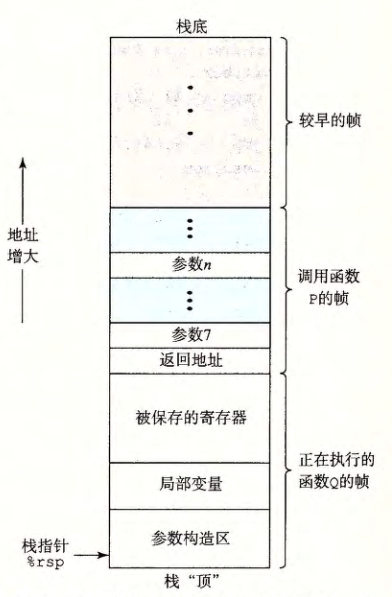
\includegraphics[width=0.4\textwidth]{stack-structure.png}
\end{figure}

\subsubsection{转移控制}

将控制从函数P转移到函数Q只需要简单地把程序计数器设置为Q的代码的起始位置。
不过,当稍后从Q返回的时候,处理器必须记录好它需要继续P的执行的代码位置。

\begin{table}[H]
    \centering
    \begin{tabular}{|c c|c|}
        \hline
        \multicolumn{2}{|c|}{\textbf{指令}} & \textbf{描述}            \\
        \hline
        call                              & Label       & 过程调用     \\
        call                              & *Operand    & 过程调用     \\
        \hline
        ret                               &             & 从过程调用中返回 \\
        \hline
    \end{tabular}
\end{table}

\subsubsection{数据传送}

当调用一个过程时,除了要把控制传递给它并在过程返回时再传递回来之外,过程调用还可能包括把数据作为参数传递。
x86-64中,可以通过寄存器最多传递6个整型(例如整数和指针)参数,大部分过程间的数据传送是通过寄存器实现的。

寄存器的使用是有特殊顺序的,寄存器使用的名字取决于要传递的数据类型的大小。

\begin{table}[H]
    \centering
    \begin{tabular}{|c|c|c|c|c|c|c|}
        \hline
        \multirow{2}{*}{\textbf{操作数大小(位)}} & \multicolumn{6}{c|}{\textbf{参数数量}}                                         \\
        \cline{2-7}
                                           & 1                                  & 2     & 3     & 4     & 5     & 6     \\
        \hline
        64                                 & \%rdi                              & \%rsi & \%rdx & \%rcx & \%r8  & \%r9  \\
        \hline
        32                                 & \%edi                              & \%esi & \%edx & \%ecx & \%r8d & \%r9d \\
        \hline
        16                                 & \%di                               & \%si  & \%dx  & \%cx  & \%r8w & \%r9w \\
        \hline
        8                                  & \%dil                              & \%sil & \%dl  & \%cl  & \%r8b & \%r9b \\
        \hline
    \end{tabular}
\end{table}

如果一个函数有大于6个整型参数,超出6个的部分就要通过栈来传递。

\paragraph{栈上的局部存储}

有些时候,局部数据必须存放在内存中,常见的情况包括:
\begin{itemize}
    \item 寄存器不足够存放所有的本地数据。
    \item 对一个局部变量使用地址运算符‘&’,因此必须能够为它产生一个地址。
    \item 某些局部变量是数组或结构,因此必须能够通过数组或结构引用被访问到。
\end{itemize}

\paragraph{寄存器中的局部存储空间}

寄存器组是唯一被所有过程共享的资源,我们需要确保当一个过程(调用者)调用另一个过程(被调用者)时,被调用者不会覆盖调用者稍后会使用的寄存器值。

根据惯例,寄存器rbx、rbp和r12-r15被划分为\emph{被调用者保存寄存器}。
当过程P调用过程Q时,Q必须保存这些寄存器的值,保证它们的值在Q返回到P时与Q被调用时是一样的。
所有其他的寄存器,除了栈指针rsp,都分类为\emph{调用者保存寄存器}。

\subsection{数据结构}
\subsubsection{数组}
对于数据类型T和整型常数N,数组声明如下:
\begin{lstlisting}[style=CStyle]
    T A[N];
\end{lstlisting}

它在内存中分配一个$L\cdot N$字节的连续区域,这里$L$是数据类型$T$的大小(单位为字节)。并且,它引入了标识符$A$,可以用$A$来
作为指向数组开头的指针,这个指针的值就是$x_A$。可以用 $0 \sim N-1$ 的整数索引来访问该数
组元素。数组元素$i$会被存放在地址为$X_A+L \cdot i$的地方。

\paragraph{指针运算}

C语言允许对指针进行运算,而计算出来的值会根据该指针引用的数据类型的大小进
行伸缩。也就是说,如果$p$是一个指向类型为$T$的数据的指针,$p$的值为$x_p$,那么表达式
$p+i$的值为$x_p+L\cdot i$,这里$L$是数据类型$T$的大小。

\paragraph{多维数组}
以二维数组为例,声明如下:
\begin{lstlisting}[style=CStyle]
    T D[R][C];
\end{lstlisting}

其元素$D[i][j]$的内存地址为
$$\&D[i][j] = x_D + L \cdot (C \cdot i + j)$$

这里$L$是数据类型$T$的大小,$x_D$是数组$D$的起始地址。

\paragraph{定长数组}
C语言编译器能够优化定长多维数组上的操作代码。
\begin{lstlisting}[style=CStyle]
/* Get element a[i][j] */
int fix_ele(fix_matrix a, size_t i, size_t j) {
    return a[i][j];
}
\end{lstlisting}
\begin{lstlisting}[style=ASMStyle]
; a in %rdi, i in %rsi, j in %rdx
salq    $6, %rsi             ; %rsi = i * 64
addq    %rsi, %rdi           ; %rdi = a + 64*i
movl    (%rdi,%rdx,4), %eax  ; %eax = M[a + 64*i + 4*j]
ret
\end{lstlisting}
\paragraph{变长数组}
历史上,C语言只支持大小在编译时就能确定的多维数组,直到ISO C99引入了一种功能,允许数组的维度是表达式,在数组被分配的时候才计算出来。
\begin{lstlisting}[style=CStyle]
/* Get element a[i][j] */
int var_ele(size_t n, int a[n][n], size_t i, size_t j) {
    return a[i][j];
}
\end{lstlisting}
\begin{lstlisting}[style=ASMStyle]
; n in %rdi, a in %rsi, i in %rdx, j in %rcx
imulq   %rdx, %rdi           ; n*i
leaq    (%rsi,%rdi,4), %rax  ; a + 4*n*i
movl    (%rax,%rcx,4), %eax  ; a + 4*n*i + 4*j
ret
\end{lstlisting}
\subsubsection{结构}
C语言的struct声明创建一个数据类型,将可能不同类型的对象聚合到一个对象中,用名字来引用结构的各个组成部分。
结构的所有组成部分都存放在内存中一段连续的区域内,而指向结构的指针就是结构第一个字节的地址。

编译器维护关于每个结构类型的信息,指示每个字段的字节偏移。
它以这些偏移作为内存引用指令中的位移,从而产生对结构元素的引用。
\begin{lstlisting}[style=CStyle]
struct s {
    int i;
    int j;
    int a[2];
    int *p;
};
\end{lstlisting}

这个结构包括4个字段:两个4字节int,一个由两个类型为int的元素组成的数组和一个8字节整型指针,总共是24个字节。

\paragraph{数据对齐}
许多计算机系统对基本数据类型的合法地址做出了一些限制,要求某种类型对象的地址必须是某个值K(通常是2、4或8)的倍数。
这种对齐限制简化了形成处理器和内存系统之间接口的硬件设计。

对齐原则是任何K字节的基本对象的地址必须是K的倍数。

\subsubsection{联合}
C语言的union声明创建一个数据类型,它的所有字段都存放在同一段内存区域中。一个联合的总的大小等于它最大字段的大小。
\begin{lstlisting}[style=CStyle]
union u {
    int i;
    float f;
    char c;
};
\end{lstlisting}

\subsubsection{浮点数}
在AVX浮点体系结构中,允许数据存储在16个YMM寄存器中,它们的名字为\%ymm0-\%ymm15。每个YMM寄存器都是256位(32字节)。
汇编代码用寄存器的SSE XMM寄存器名字\%xmm0-\%xmm15来引用它们,每个XMM寄存器都是对应的YMM寄存器的低128位(16字节)。
\paragraph{传送指令}
\begin{table}[H]
    \centering
    \begin{tabular}{|c c|c|}
        \hline
        \multicolumn{2}{|c|}{\textbf{指令}} & \textbf{描述}                 \\
        \hline
        vmovss                            & M$_{32}$, X & 传送单精度数        \\
        \hline
        vmovss                            & X, M$_{32}$ & 传送单精度数        \\
        \hline
        vmovsd                            & M$_{64}$, X & 传送双精度数        \\
        \hline
        vmovsd                            & X, M$_{64}$ & 传送双精度数        \\
        \hline
        vmovaps                           & X, X        & 传送对齐的封装好的单精度数 \\
        \hline
        vmovapd                           & X, X        & 传送对齐的封装好的双精度数 \\
        \hline
    \end{tabular}
\end{table}

\paragraph{转换指令}
\begin{table}[H]
    \centering
    \begin{tabular}{|c c|c|}
        \hline
        \multicolumn{2}{|c|}{\textbf{指令}} & \textbf{描述}                               \\
        \hline
        vcvttss2si                        & X/M$_{32}$, R$_{32}$ & 用截断的方法把单精度数转换成整数   \\
        \hline
        vcvttsd2si                        & X/M$_{64}$, R$_{32}$ & 用截断的方法把双精度数转换成整数   \\
        \hline
        vcvttsd2si                        & X/M$_{64}$, R$_{32}$ & 用截断的方法把双精度数转换成整数   \\
        \hline
        vcvttss2siq                       & X/M$_{32}$, R$_{64}$ & 用截断的方法把单精度数转换成四字整数 \\
        \hline
        vcvttsd2siq                       & X/M$_{64}$, R$_{64}$ & 用截断的方法把双精度数转换成四字整数 \\
        \hline
    \end{tabular}
\end{table}
\begin{table}[H]
    \centering
    \begin{tabular}{|c c|c|}
        \hline
        \multicolumn{2}{|c|}{\textbf{指令}} & \textbf{描述}                            \\
        \hline
        vcvtssi2ss                        & M$_{32}$/R$_{32}$, X, X & 把整数转换成单精度数   \\
        \hline
        vcvtssi2sd                        & M$_{32}$/R$_{32}$, X, X & 把整数转换成双精度数   \\
        \hline
        vcvtssi2ssq                       & M$_{64}$/R$_{64}$, X, X & 把四字整数转换成单精度数 \\
        \hline
        vcvtssi2sdq                       & M$_{64}$/R$_{64}$, X, X & 把四字整数转换成双精度数 \\
        \hline
    \end{tabular}
\end{table}
\paragraph{运算指令}
每条指令有一个($S_1$)或两个($S_1$, $S_2$)源操作数,和一个目的操作数$D$。第一个源操作数$S_1$可以是一个XMM寄存器
或一个内存位置,第二个源操作数和目的操作数都必须是XMM寄存器。
\begin{table}[H]
    \centering
    \begin{tabular}{|c|c|c|c|c|c|}
        \hline
        \multicolumn{4}{|c|}{\textbf{指令}} & \textbf{效果} & \textbf{描述}                                                   \\
        \hline
        vaddss                            & vaddsd      & vaddps      & vaddpd & $D \leftarrow S_2 + S_1$      & 浮点数加   \\
        \hline
        vsubss                            & vsubsd      & vsubps      & vsubpd & $D \leftarrow S_2 - S_1$      & 浮点数减   \\
        \hline
        vmulss                            & vmulsd      & vmulps      & vmulpd & $D \leftarrow S_2 \times S_1$ & 浮点数乘   \\
        \hline
        vdivss                            & vdivsd      & vdivps      & vdivpd & $D \leftarrow S_2 / S_1$      & 浮点数除   \\
        \hline
        vmaxss                            & vmaxsd      & vmaxps      & vmaxpd & $D \leftarrow \max(S_2, S_1)$ & 浮点数最大值 \\
        \hline
        vminss                            & vminsd      & vminps      & vminpd & $D \leftarrow \min(S_2, S_1)$ & 浮点数最小值 \\
        \hline
        sqrtss                            & sqrtsd      & sqrtps      & sqrtpd & $D \leftarrow \sqrt{S_1}$     & 浮点数平方根 \\
        \hline
        vxorss                            & vxorsd      & vxorps      & vxorpd & $D \leftarrow S_2 \oplus S_1$ & 位级异或   \\
        \hline
        vandss                            & vandsd      & vandps      & vandpd & $D \leftarrow S_2 \& S_1$     & 位级与    \\
        \hline
    \end{tabular}
\end{table}

\paragraph{比较指令}
\begin{table}[H]
    \centering
    \begin{tabular}{|c c|c|}
        \hline
        \multicolumn{2}{|c|}{\textbf{指令}} & \textbf{描述}          \\
        \hline
        ucomiss                           & $S_1, S_2$  & 比较单精度值 \\
        \hline
        ucomisd                           & $S_1, S_2$  & 比较双精度值 \\
        \hline
    \end{tabular}
\end{table}

浮点比较指令会设置三个条件码:零标志位ZF、进位标志位CF和奇偶标志位PF。对于整数
操作,当最近的一次算术或逻辑运算产生的值的最低位字节是偶校验的(即这个字节中有
偶数个1),就会设置PF标志位。不过对于浮点比较,当两个操作数中任一个是
NaN时,会设置该位。
\begin{table}[H]
    \centering
    \begin{tabular}{|c|c|c|c|}
        \hline
        顺序 $S_2:S_1$ & CF & ZF & PF \\
        \hline
        无序的          & 1  & 1  & 1  \\
        \hline
        $S_2 < S_1$  & 1  & 0  & 0  \\
        \hline
        $S_2 = S_1$  & 0  & 1  & 0  \\
        \hline
        $S_2 > S_1$  & 0  & 0  & 0  \\
        \hline
    \end{tabular}
\end{table}


\subsection{机器级程序进阶}
\subsubsection{类型声明}

右左法则:首先从标识符看起,然后往右看,再往左看。每当遇到圆括号时,就应该掉转阅读方向。一旦解析完圆括号里面所有的东西,就跳出圆括号。重复这个过程直到整个声明解析完毕。
\begin{lstlisting}[style=CStyle]
int * (* (*a) (int) ) [10];
/*
阅读步骤:
1. 从变量名开始:a
2. 往右看,什么也没有,碰到了')',因此往左看,碰到一个'*':一个指针
3. 跳出括号,碰到了(int):一个带一个int参数的函数
4. 向左看,发现一个'*':(函数)返回一个指针
5. 跳出括号,向右看,碰到[10]:一个10元素的数组
6. 向左看,发现一个'*':指针
7. 向左看,发现int:int类型
总结:a被声明成为一个函数的指针,该函数返回指向指针数组的指针
*/
\end{lstlisting}

\subsubsection{内存布局}
\begin{figure}[H]
    \centering
    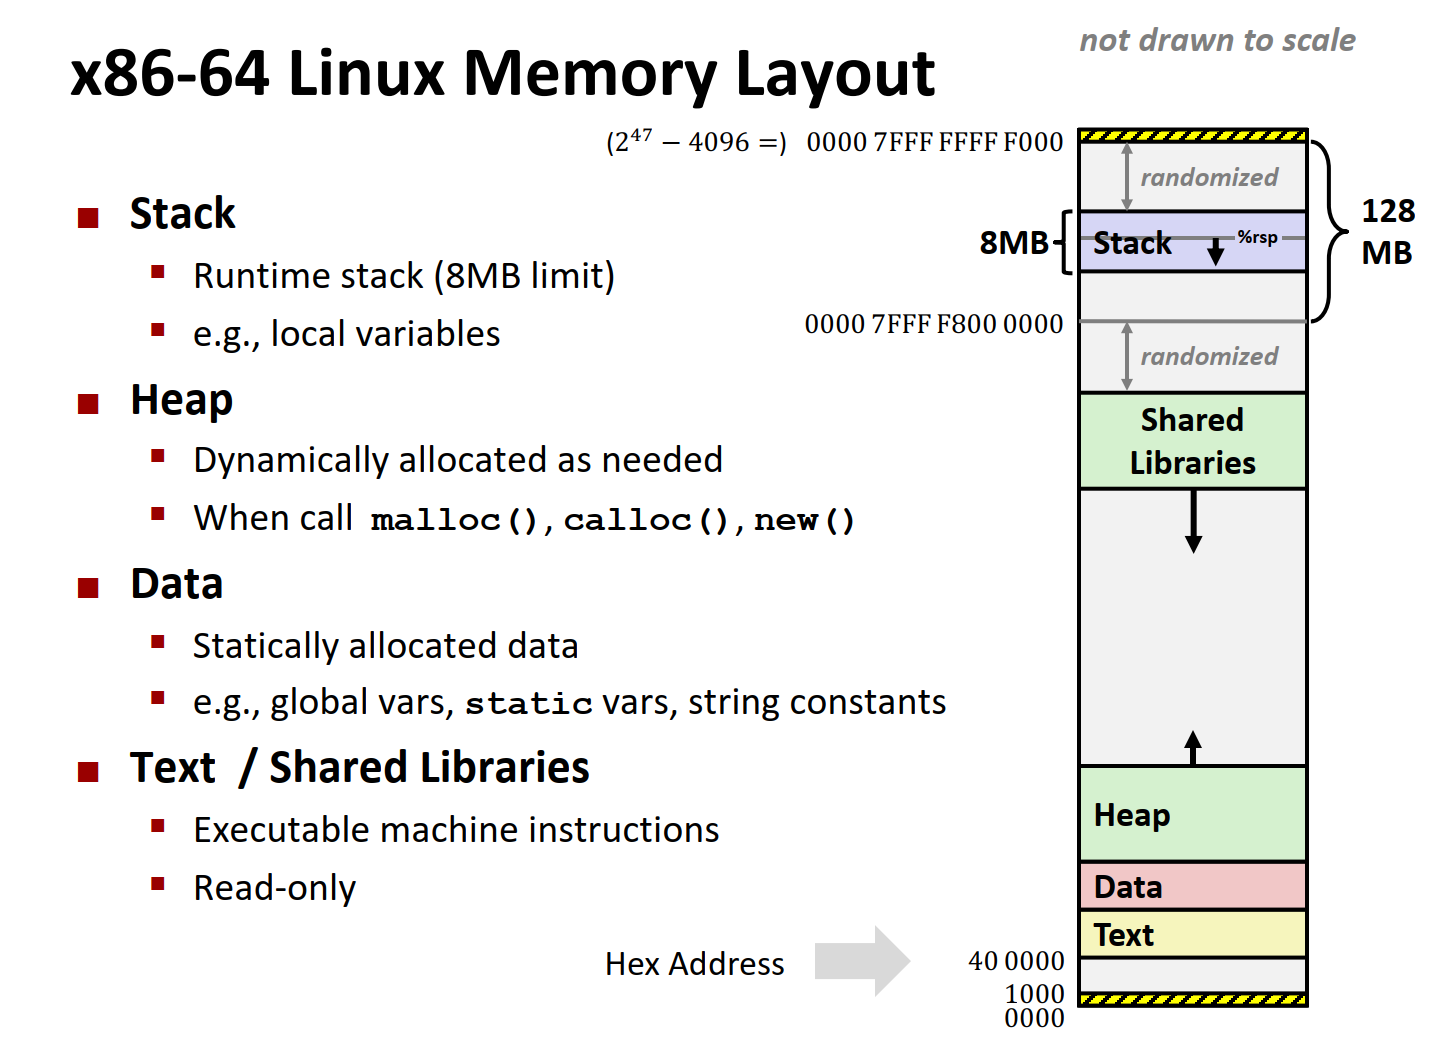
\includegraphics[width=\textwidth]{memory-layout.png}
\end{figure}

\subsubsection{缓冲溢出攻击}
C对于数组引用不进行任何边界检查,而且局部变量和状态信息(例如保存的寄存器值和返回地址)都存放在栈中。
对越界的数组元素的写操作可能会破坏存储在栈中的状态信息。

一种特别常见的状态破坏称为\emph{缓冲区溢出}。
\begin{lstlisting}[style=CStyle]
/* Implementation of library function gets() */
char *gets(char *s)
{
    int c;
    char *dest = s;
    while ((c = getchar()) != '\n' && c != EOF)
        *dest++ = c;
    if (c == EOF && dest == s)
        /* No characters read */
        return NULL;
    *dest++ ='\0';  /* Terminate string */
    return s;
}
/* Read input line and write it back */
void echo()
{
    char buf[8];  /* Way too small! */
    gets(buf);
    puts(buf);
}
\end{lstlisting}
\begin{lstlisting}[style=ASMStyle]
; void echo()
echo:
subq    $24, %rsp
movq    %rsp, %rdi
call    gets
movq    %rsp, %rdi
call    puts
addq    $24, %rsp
ret
\end{lstlisting}
\paragraph{栈粉碎攻击}

汇编代码显示,函数调用的参数和存储的返回指针之间的16个字节是未被使用的。
只要用户输入不超过7个字符,gets返回的字符串(包括结尾的null) 就能够放进为buf分配的空间里。
不过,长一些的字符串就会导致gets覆盖栈上存储的某些信息。
随着字符串变长,下面的信息会被破坏:
\begin{table}[H]
\centering
\begin{tabular}{|c|c|}
\hline
输入的字符数量 & 附加的被破坏的状态 \\ \hline
0到7                               & 无                                      \\ \hline
9到23                              & 未被使用的栈空间                        \\ \hline
24到31                             & 返回地址                                \\ \hline
32及以上                               & caller中保存的状态                      \\ \hline
\end{tabular}
\end{table}

字符串到23个字符之前都没有严重的后果,但是超过以后,返回指针的值以及更多可能的保存状态会被破坏。
如果存储的返回地址的值被破坏了,那么ret指令会导致程序跳转到一个完全意想不到的位置。

\paragraph{代码注入攻击}

缓冲区溢出的一个更加致命的使用就是让程序执行它本来不愿意执行的函数。
这是一种最常见的通过计算机网络攻击系统安全的方法。

通常,输入给程序一个字符串,这个字符串包含一些可执行代码的字节编码,称为攻击代码。
另外,还有一些字节会用一个指向攻击代码的指针覆盖返回地址。
那么,执行ret指令的效果就是跳转到攻击代码。
\begin{figure}[H]
    \centering
    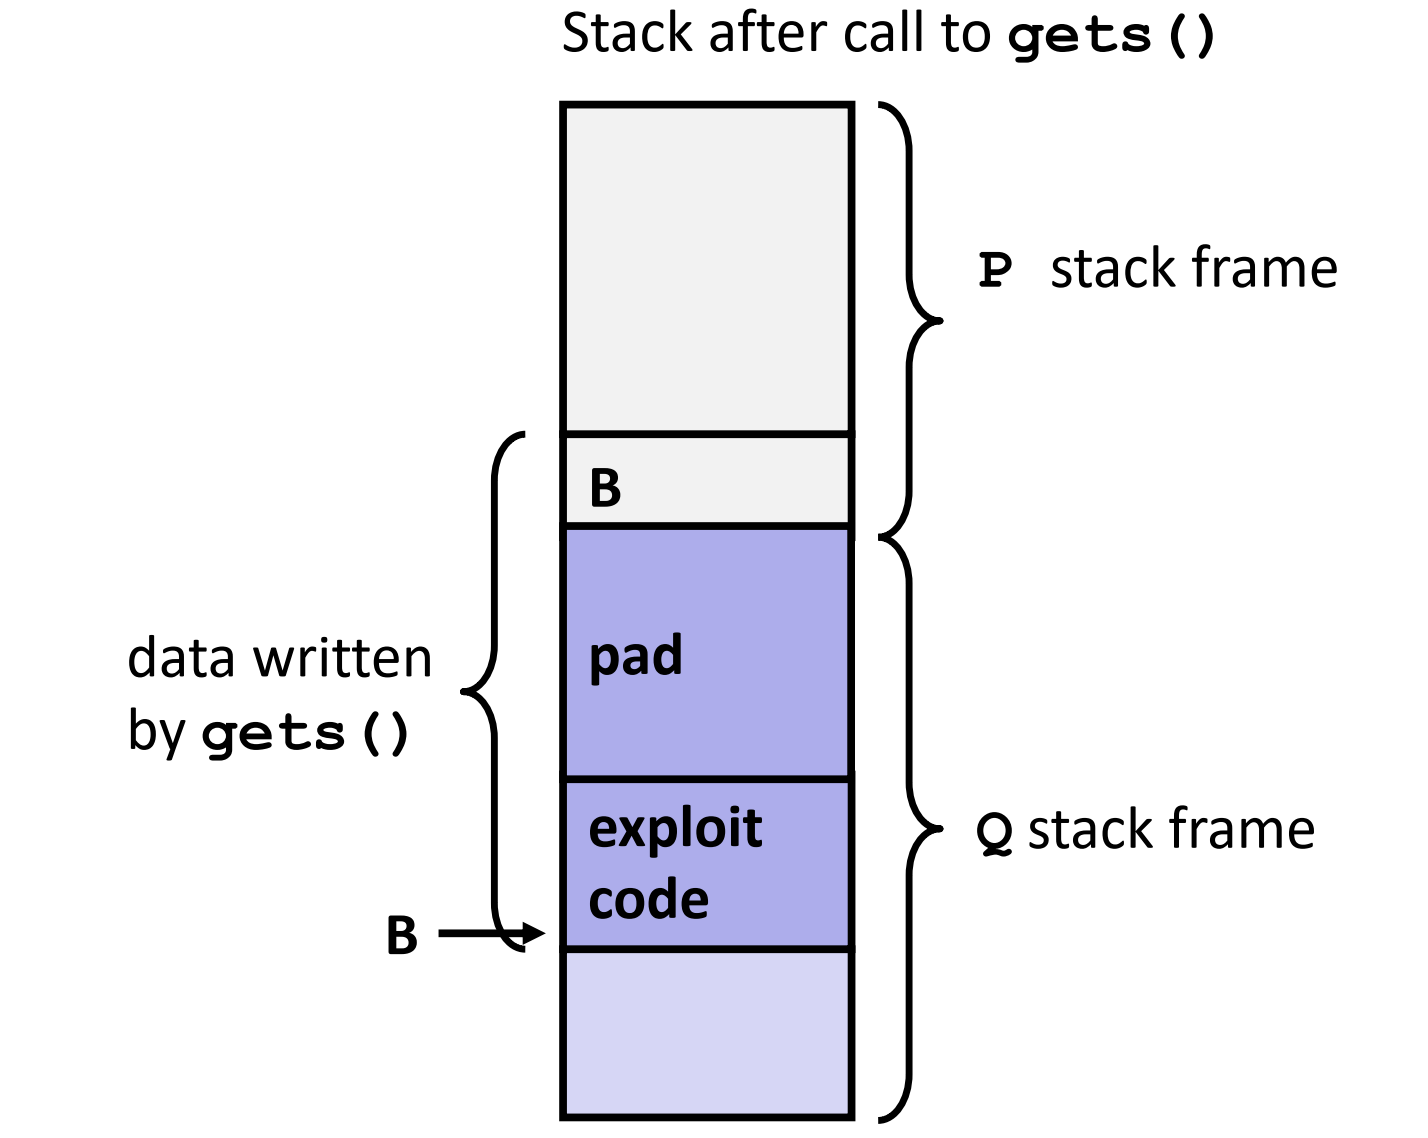
\includegraphics[width=0.6\textwidth]{code-injection-attacks.png}
\end{figure}

\subsubsection{缓冲溢出保护}
\paragraph{代码级保护}
通常,使用gets或其他不检查目标缓冲区大小的函数很容易导致溢出。
为了避免这类问题,应优先使用带长度限制的替代函数,例如
用fgets(buf, sizeof buf, stdin)或POSIX的getline代替gets,
用snprintf代替sprintf,
用strncat/strncpy或更推荐的BSD扩展strlcpy/strlcat来进行字符串复制和拼接。

\paragraph{栈随机化}
为了在系统中插入攻击代码,攻击者既要插入代码,也要插入指向这段代码的指针,这个指针也是攻击字符串的一部分。

产生这个指针需要知道这个字符串放置的栈地址,栈随机化的思想使得栈的位置在程序每次运行时都有变化。
因此,即使许多机器都运行同样的代码,它们的栈地址都是不同的。
实现的方式是:程序开始时,在栈上分配一段0到n字节之间的随机大小的空间。

\paragraph{限制可执行代码区域}
在典型的程序中,只有保存编译器产生的代码的那部分内存才需要是可执行的,其他部分应当被限制为只允许读和写。
随着处理器的内存保护引入了"NX"位,将读和执行访问模式分开,栈可以被标记为可读和可写,但是不可执行。
由此,攻击代码即使被插入到栈中,也无法被执行。

\paragraph{栈破坏检测}
在C语言中,没有可靠的方法来防止对数组的越界写。
但是,我们能够在发生了越界写的时候,在造成任何有害结果之前,尝试检测到它。

较新版本的GCC在产生的代码中加入了一种栈保护者机制。
该机制通过在栈帧中插入一个金丝雀值(canary)来检测栈溢出。
在函数调用时,GCC会生成代码来保存当前的金丝雀值,并在函数返回时检查它是否被修改。
如果金丝雀值被篡改,程序会立即终止,从而防止潜在的攻击。

\begin{lstlisting}[style=ASMStyle]
my_function:
    pushq   %rbp                    ; 保存旧的基指针
    movq    %rsp, %rbp              ; 建立新的栈帧
    subq    $32, %rsp               ; 为局部变量与保存区留出空间
    movq    %fs:40, %rax            ; 段寻址读取金丝雀值
    movq    %rax, -8(%rbp)          ; 将金丝雀值保存到栈帧
    ; ... 函数的实际主体 ...
    movq    -8(%rbp), %rax          ; 从栈中取出保存的金丝雀值
    cmpq    %fs:40, %rax            ; 将其与当前金丝雀值比较
    jne     .Lstack_chk_fail        ; 若不相等,跳转到失败处理
    addq    $32, %rsp               ; 清理栈上分配
    popq    %rbp                    ; 恢复旧的基指针
    ret
.Lstack_chk_fail:
    callq   __stack_chk_fail@plt
\end{lstlisting}

\newpage